\documentclass[cjk,slidestop,compress,mathserif,blue]{beamer}
%dvipdfm选项是关键,否则编译统统通不过
%beamer的颜色选项定义的是导航条和标题的颜色(即关键词structure的颜色)

%%%%%%%%%%%%%%%%仅限于XeTeX可使用的宏包%%%%%%%%%%%%%%%%%%%%%%%%%%%%
\usepackage{fontspec,xunicode,xltxtra,beamerthemesplit}
%\usepackage{beamerthemesplit}
\usepackage{xeCJK}
\setCJKmainfont[BoldFont=黑体, ItalicFont=楷体, BoldItalicFont=仿宋]{黑体}
%\setsansfont[Mapping=tex-text]{Adobe 黑体 Std}
%如果装了Adobe Acrobat,可在font.conf中配置Adobe字体的路径以使用其中文字体
%也可直接使用系统中的中文字体如SimSun,SimHei,微软雅黑 等
%原来beamer用的字体是sans family;注意Mapping的大小写,不能写错

%%%%%%%%   确定标题和导航条结构的框架     %%%%%%%%%%%%
\usepackage{beamerthemeshadow}                       %
%\usepackage{beamerthemeclassic}%导航条色与背景色一致%
%%%%%%%%%%%%%%%%%%%%%%%%%%%%%%%%%%%%%%%%%%%%%%%%%%%%%%
\setbeamerfont{roman title}{size={}}
%\usepackage{CJK} % CJK 中文支持                                  %
\usepackage{amsmath,amsthm,amsfonts,amssymb,bm}
\usepackage{mathrsfs}
\usepackage{xcolor}                                        %使用默认允许使用颜色
\usepackage{hyperref} 
\usepackage{graphicx}
\usepackage{subfigure}           %图片跨页

%\usepackage[numbers,sort&compress]{natbib} %紧密排列             %
\usepackage[sectionbib]{chapterbib}        %每章节单独参考文献   %
\usepackage{hypernat}                                                                         %
%\usepackage[dvipdfm,bookmarksopen=true,pdfstartview=FitH,CJKbookmarks]{hyperref}		%
\hypersetup{bookmarksnumbered,colorlinks,linkcolor=brown,citecolor=blue,urlcolor=red}         %
%参考文献含有超链接引用时需要下列宏包,注意与natbib有冲突        %
%\usepackage[dvipdfm]{hyperref}                                  %
%\usepackage{hypernat}                                           %
\newcommand{\upcite}[1]{\hspace{0ex}\textsuperscript{\cite{#1}}} %

%\useoutertheme{smoothbars}
\useinnertheme[shadow=true]{rounded}
\usetheme{Berkeley}                                          %主题式样
%\usetheme{Luebeck}

\usecolortheme{lily}                                        %颜色主题式样

\usefonttheme{professionalfonts}                           %字体主题样式宏包

%\beamertemplatetransparentcoveredhigh                      %使所有被隐藏的文本高度透明
\beamertemplatetransparentcovereddynamicmedium             %使所有被隐藏的文本完全透明,动态,动态的范围很小
\mode<presentation>
%\beamersetaveragebackground{gray}                          %设置背景颜色(单一色) 
\beamertemplateshadingbackground{green!10}{red!5}         %设置背景颜色(渐变色)

%i放置单位logo
%\logo{
\includegraphics[width=1.6cm,height=0.35cm]{Figures/BCC_logo-1.png}}	%简单设置logo

%\pgfdeclareimage[width=3.5cm]{logoname}{Figures/BCC_logo-1.png}		%logo置于左侧微调
%\logo{\pgfuseimage{logoname}{\vspace{0.2cm}\hspace*{-2.0cm}}}

%在指定位置精确放置logo
\usepackage{tikz}
\usepackage{beamerfoils}
\usepackage{pgf}
\logo{\pgfputat{\pgfxy(11.68,0.15)}{
\includegraphics[height=1.01cm,viewport=0 0 140 120,clip]{Figures/BCC_logo-1.png}}\pgfputat{\pgfxy(10.502,-0.218)}{
\includegraphics[height=0.369cm,viewport=140 0 540 120,clip]{Figures/BCC_logo-1.png}}}
%\logo{\pgfputat{\pgfxy(11.68,0.15)}{
\includegraphics[height=0.95cm,viewport=0 0 510 360,clip]{Figures/Logo_Gainstrong.png}}\pgfputat{\pgfxy(10.333,-0.195)}{
\includegraphics[height=0.35cm,viewport=530 70 1100 218,clip]{Figures/Logo_Gainstrong.png}}}
%\MyLogo{
%	\pgfputat{\pgfxy(-50,-50)}{\pgfbox[right,base]{
\includegraphics[height=1cm]{Figures/BCC_logo-1.png}}}

%logo作为背景放置
%\setbeamertemplate{background}{
%	\pgfputat{\pgfxy(6.5,-0.5)}{\pgfbox[left,top]{\pgfimage[height=1.1cm]{Figures/BCC_logo-1.png}}}}

%\logo{}									%不显示logo

\begin{document}
%\begin{CJK*}{GBK}{song}
%\begin{CJK*}{GBK}{kai}
%beamer下不能用\songyi、\zihao等命令!
%\graphicspath{Figures/}

%-------------------------------PPT Title-------------------------------------
\title{Green's function~和GW~方法}
%-----------------------------------------------------------------------------

%----------------------------Author & Date------------------------------------
\author{北京市计算中心\;云平台\:姜骏}
\date{\textrm{2017.01.11}}
%\date{2013.09.10}
\frame{\titlepage}
%-----------------------------------------------------------------------------

%------------------------------------------------------------------------------列出全文 outline ---------------------------------------------------------------------------------
\section*{}
\frame[allowframebreaks]
{
  \frametitle{Outline}
%  \frametitle{\textcolor{mycolor}{\secname}}
  \tableofcontents%[current,currentsection,currentsubsection]
}
%在每个section之前列出全部Outline
%类似的在每个subsection之前列出全部Outline是\AtBeginSubsection[]
\AtBeginSection[]
{
  \frame<handout:0>
  {
    \frametitle{Outline}
%全部Outline中,本部分加亮
    \tableofcontents[current,currentsection]
  }
}

%------------------------------------------------------------------------------PPT main Body------------------------------------------------------------------------------------
\small
\section{\rm{Green's function}}
\frame
{
	\frametitle{\textrm{Green's function}}
	\textrm{Green's function~}方法是求解常微分方程和偏微分方程常用方法,\textcolor{blue}{以求解\textrm{Poisson~}方程为例}
		\vskip -10pt		
		\begin{displaymath}
			\nabla^2\phi(\vec r)=-\frac1{\varepsilon_0}\rho_e(\vec r)
		\end{displaymath}
		引入相关的简单微分方程
		\vskip -10pt		
		\begin{displaymath}
			\nabla_{\vec r}G(\vec r)=\delta(\vec r)
		\end{displaymath}
		这里$G(\vec r)$是\textrm{Laplace~}算符$\nabla_{\vec r}$的\textrm{Green's function},有
		\vskip -8pt		
		\begin{displaymath}
			\phi(\vec r)=-\frac1{\varepsilon_0}\int\mathrm{d}\vec r^{\prime}G(\vec r-\vec r^{\prime})\rho_e(\vec r^{\prime})
		\end{displaymath}
		对$G(\vec r)$作\textrm{Fourier~}变换$-k^2G(\vec k)=1\Rightarrow G(\vec k)=-\frac1{k^2}$,有
		\vskip -5pt		
		\begin{displaymath}
				G(\vec r)=\int\frac{\mathrm{d}\vec r}{(2\pi)^3}\mathrm{e}^{\mathrm{i}\vec k\cdot\vec r}G(\vec k)=-\int\frac{\mathrm{d}\vec k}{(2\pi)^3}\frac{\mathrm{e}^{\mathrm{i}\vec k\cdot\vec r}}{k^2}=-\frac1{4\pi r}
		\end{displaymath}
		因此
		\vskip -5pt		
		\begin{displaymath}
			\phi(\vec r)=\frac1{4\pi\varepsilon_0}\int\mathrm{d}\vec r^{\prime}\frac{\rho_e(\vec r^{\prime})}{|\vec r-\vec r^{\prime}|}
		\end{displaymath}
}

\frame
{
	\frametitle{单粒子\textrm{Schr\"odinger~}方程的\textrm{Green's function}}
	\textcolor{violet}{\textrm{Green's function~}在微扰理论求解中特别有用}\\例如对于\textrm{Schr\"odinger~}方程
	\begin{displaymath}
		[H_0(\vec r)+V(\vec r)]\Psi_E=E\Psi_E
	\end{displaymath}
	如果已知$H_0$的本征态,而将$V$视作微扰\\
	(\textcolor{blue}{对应于散射理论中的图像:~一束入射粒子(由$H_0$描述)与体系中势能$V$发生相互作用后,粒子将处于不同的出射状态})
	\vskip 10pt
	为求解\textrm{Schr\"odinger~}方程,定义\textrm{Green's function~}相关的微分方程
	\begin{displaymath}
		[E-H_0(\vec r)]G_0(\vec r,\vec r^{\prime};E)=\delta(\vec r-\vec r^{\prime})
	\end{displaymath}
	有边条件$G_0(\vec r,\vec r^{\prime})=G_0(\vec r^{\prime},\vec r)$,因此
	\begin{displaymath}
		G_0^{-1}(\vec r,E)=E-H_0(\vec r)
	\end{displaymath}
	因此\textrm{Schr\"odinger~}方程可表示为
	\begin{displaymath}
		[G_0^{-1}(\vec r,E)-V(\vec r)]\Psi_E=0
	\end{displaymath}
}

\frame
{
	\frametitle{单粒子\textrm{Schr\"odinger~}方程的\textrm{Green's function}}
	积分方程形式的\textrm{Schr\"odinger~}方程解
	\begin{displaymath}
		\Psi_E(\vec r)=\Psi_E^0(\vec r)+\int\mathrm{d}\vec r^{\prime}G_0(\vec r,\vec r^{\prime};E)V(\vec r^{\prime})\Psi_E(\vec r^{\prime})
	\end{displaymath}
	\textcolor{red}{写成迭代求解形式}
	\begin{displaymath}
		\begin{aligned}
			\Psi=&\Psi^0+G_0V\Psi_0+G_0VG_0V\Psi^0+G_0VG_0VG_0V\Psi^0+\cdots\\
			=&\Psi^0+(G_0+G_0VG_0+G_0VG_0VG_0+\cdots)V\Psi^0
		\end{aligned}
	\end{displaymath}
	因此完整的\textrm{Green's function~}$G$可以表示为
	\begin{displaymath}
		\begin{aligned}
			G=&G_0V+G_0VG_0V+G_0VG_0VG_0V+\cdots\\
			=&G_0+G_0V(G_0+G_0VG_0+\cdots)
		\end{aligned}
	\end{displaymath}
	由此可得\textrm{Dyson~}方程
	\begin{displaymath}
		G=G_0+G_0VG
	\end{displaymath}
}

\section{\rm{Green's function~}与自能}
\frame
{
	\frametitle{单粒子图像的缺陷}
	\begin{itemize}
		\item 梯度校正近似(\textrm{GGA})\textcolor{blue}{主要关注总能$E_{\mathrm{TOT}}$的修正},但没有注意对准粒子能量本征值改进
		\item 自相互作用校正(\textrm{SIC})\textcolor{blue}{只改善局域轨道能量本征值},对离域电子体系的带隙没有改进
		\item \textrm{LDA}+$U$\textcolor{blue}{适用于过渡金属氧化物},但用于过渡金属体系计算结果不合理
		\item 杂化泛函中\textcolor{blue}{精确交换泛函的引入导致计算量大},没有考虑动态相关
	\end{itemize}
	\textrm{GWA~}是根据多体微扰理论(\textrm{Many-Body perturbation theory, MBPT})发展起来,其自能(\textrm{Self-energt})的特征
	\begin{enumerate}
		\item \textcolor{red}{考虑了电子的\textrm{Coulomb~}相互作用的动态屏蔽}
		\item \textcolor{red}{非局域且与能量相关}
	\end{enumerate}
	\textrm{GWA~}主要用于计算单粒子激发谱
}
\frame
{
	\frametitle{\textrm{Green's function~}与自能}
		由二次量子化理论,含时单粒子\textrm{Green's function}的定义
	\begin{displaymath}
		\mathrm{i}G(\mathbf{x},\mathbf{x}^{\prime})=\langle N|T[\hat\psi(\mathbf{x})\hat\psi^{\dag}(\mathbf{x}^{\prime})]|N\rangle=\left\{
		\begin{aligned}
			&\langle N|\hat\psi(\mathbf{x})\hat\psi^{\dag}(\mathbf{x}^{\prime})|N\rangle\\
			&-\langle N|\hat\psi^{\dag}(\mathbf{x}^{\prime})\hat\psi(\mathbf{x})|N\rangle
		\end{aligned}
		\right.
	\end{displaymath}
	这里$|N\rangle$是$N$-粒子基态,$\hat\psi(\mathbf{x})$是场算符的\textrm{Heisenberg~}表示,$\mathbf{x}=(\vec r,x)$,$T$是时间序列算符
	\vskip 5pt
	\textrm{Green's function}的\textcolor{blue}{物理意义:~}\\
	\begin{itemize}
		\item 当$t^{\prime}>t$,表示\textcolor{violet}{时空点$\mathbf{x}$产生的空穴向点$\mathbf{x^{\prime}}$传播}
		\item 当$t>t^{\prime}$,表示\textcolor{violet}{时空点$\mathbf{x}^{\prime}$放入的电子向$\mathbf{x}$传播}
	\end{itemize}
	根据\textrm{Heisenberg~}运动方程,对于场算符
	\begin{displaymath}
		\mathrm{i}\frac{\partial\hat\psi\mathbf(x)}{\partial t}=[\hat\psi(\mathbf{x}),\hat H]
	\end{displaymath}
	\vskip -5pt
	\fontsize{8.5pt}{6.2pt}\selectfont{其中\textrm{Hamiltonian~}$\hat H$的二次量子化表示为
	\vskip -8pt
	\begin{displaymath}
	\hat H=\int\mathrm{d}^3r\hat{\psi}^{\dag}(\mathbf{x})h_0(\mathbf{x})\hat{\psi}(\mathbf{x})+\frac12\int\mathrm{d}^3r\mathrm{d}^3r^{\prime}\hat{\psi}^{\dag}(\vec r,t)\hat{\psi}^{\dag}(\vec r^{\prime},t)v(\vec r-\vec r^{\prime})\hat{\psi}(\vec r^{\prime},t)\hat{\psi}(\vec t,r)
	\end{displaymath}}
}

\frame
{
	\frametitle{\textrm{Green's function~}与自能}
	\textrm{Green's function~}的运动方程
	\begin{displaymath}
		\left[ \mathrm{i}\frac{\partial}{\partial t}-h_0(\mathbf{x}) \right]G(\mathbf{x},\mathbf{x}^{\prime})-\int\mathrm{d}\mathbf{x}^{\prime\prime}M(\mathbf{x},\mathbf{x}^{\prime\prime})G(\mathbf{x}^{\prime\prime},\mathbf{x}^{\prime})=\delta(\mathbf{x}-\mathbf{x}^{\prime})
	\end{displaymath}
	其中质量算符$M$(\textrm{Hartree~}势+自能(\textrm{self-energy}))的定义
	\begin{displaymath}
		\begin{aligned}
			&\int\mathrm{d}\mathbf{x}_1M(\mathbf{x},\mathbf{x}_1)G(\mathbf{x}_1,\mathbf{x}^{\prime})\\
			=&-\mathrm{i}\int\mathrm{d}r_1v(\vec r-\vec r_1)\langle N|T[\hat{\psi}^{\dag}(\vec r_1,t)\hat{\psi}(\vec r_1,t)\hat{\psi}(\vec r,t)\hat{\psi}^{\dag}(\vec r^{\prime},t^{\prime})]|N\rangle
		\end{aligned}
	\end{displaymath}
	这里$h_0$是动能算符和局域外势之和,右侧是双粒子\textrm{Green's function},一般定义为
	\begin{displaymath}
		G_2(\mathbf{1},\mathbf{2},\mathbf{3},\mathbf{4})=(\mathrm{i})^2\langle N|T[\hat{\psi}(\mathbf{1})\hat{\psi}(\mathbf{3})\hat{\psi}^{\dag}(\mathbf{4})\hat{\psi}^{\dag}(\mathbf{2})]|N\rangle
	\end{displaymath}
	这里$\mathbf{1}\equiv\mathbf{x}_1=(\vec r_1,t_1)$
}

\frame
{
	\frametitle{\textrm{Green's function~}与自能}
	为导出自能的计算方案,引入含时变量场$\phi(\vec r,t)$\\根据相互作用表象(\textrm{Dirac~}表象)
	\begin{displaymath}
		|\psi_D(\vec r,t)\rangle=\hat{U}(t,t_0)|\psi_D(\vec r,t_0)\rangle
	\end{displaymath}
	含时变化算符$\hat U$的定义为
	\begin{displaymath}
		\begin{aligned}
			&\hat U(t,t_0)=T\mathrm{exp}\left[ -\mathrm{i}\int_{t_0}^t\mathrm{d}\tau\hat{\phi}(\tau) \right]\\
			&\hat{\phi}(\tau)=\int\mathrm{d}r\phi(\vec r,\tau)\hat{\psi}_D^{\dag}(\vec r,\tau)\hat{\psi}_D(\vec r,t)
		\end{aligned}
	\end{displaymath}
	根据\textrm{Heisenberg~}表象和\textrm{Dirac~}算符的关系,场算符可表示为
	\begin{displaymath}
		\hat{\psi}(\vec r,t)=\hat{U}^{\dag}(t,0)\hat{\psi}_D(\vec r,t)\hat{U}(t,0)
	\end{displaymath}
	并满足
	\begin{displaymath}
		\mathrm{i}\frac{\partial}{\partial t}\hat{\psi}_D=[\hat{\psi}_D,\hat{H}(\phi=0)]
	\end{displaymath}
}

\frame
{
	\frametitle{\textrm{Green's function~}与自能}
	\textrm{Green's function~}可表示为
	\begin{displaymath}
		\mathrm{i}G(\mathbf{1},\mathbf{2})=\frac{\langle N^0|T[\hat{U}(\infty,-\infty)\hat{\psi}_D(\mathbf{1})\hat{\psi}_D^{\dag}(\mathbf{2})]|N^0\rangle}{\langle N^0|\hat{U}(\infty,-\infty)|N^0\rangle}
	\end{displaymath}
	泛函$G$对$\phi$的导数
	\begin{displaymath}
		\frac{\delta G(\mathbf{1},\mathbf{2})}{\delta\phi(\mathbf{3})}=G(\mathbf{1},\mathbf{2})G(\mathbf{3},\mathbf{3}^{+})-G_2(\mathbf{1},\mathbf{2},\mathbf{3},\mathbf{3}^{+})
	\end{displaymath}
	注意到$M$和双粒子\textrm{Green's function~}的关系,且$GG$给出\textrm{Hartree~}势$V^{\mathrm H}$,因此
	\begin{displaymath}
		\Sigma=M-V^{\mathrm H}
	\end{displaymath}
	\textrm{Green's function~}的运动方程
	\begin{displaymath}
		\left[ \mathrm{i}\frac{\partial}{\partial t}-H_0(\mathbf{x}) \right]G(\mathbf{x},\mathbf{x}^{\prime})-\int\mathrm{d}\mathbf{x}^{\prime\prime}\Sigma(\mathbf{x},\mathbf{x}^{\prime\prime})G(\mathbf{x}^{\prime\prime},\mathbf{x}^{\prime})=\delta(\mathbf{x}-\mathbf{x}^{\prime})
	\end{displaymath}
	这里
	\begin{displaymath}
		H_0=h_0+V^{\mathrm H}+\phi
	\end{displaymath}
}

\frame
{
	\frametitle{\textrm{Green's function~}与自能}
	自能可表示为
	\begin{displaymath}
		\Sigma(\mathbf{1},\mathbf{2})=\mathrm{i}\int\mathrm{d}\mathbf{3}\mathrm{d}\mathbf{4}G(\mathbf{1},\mathbf{3}^{+})W(\mathbf{1},\mathbf{4})\Lambda(\mathbf{3},\mathbf{2},\mathbf{4})
	\end{displaymath}
	这里\textcolor{blue}{$W$是屏蔽\textrm{Coulomb~}势}
	\begin{displaymath}
		\begin{aligned}
			&W(\mathbf{1},\mathbf{2})=\int\mathrm{d}\mathbf{3}\epsilon^{-1}(\mathbf{1},\mathbf{3})v(\mathbf{3}-\mathbf{2})\\
			&\epsilon^{-1}(\mathbf{1},\mathbf{2})=\frac{\delta V(\mathbf{1})}{\delta\phi(\mathbf{2})}
		\end{aligned}
	\end{displaymath}
	这里$V$是\textrm{Hartree~}势和外势之和
	\begin{displaymath}
		V=V^{\mathrm H}+\phi
	\end{displaymath}
	\fontsize{8.5pt}{6.2pt}\selectfont{$\Lambda$是顶角函数(\textrm{vertex function})
	\begin{displaymath}
		\begin{aligned}
			&\Lambda(\mathbf{1},\mathbf{2},\mathbf{3})=-\frac{\delta G^{-1}(\mathbf{1},\mathbf{2})}{\delta V(\mathbf{3})}=\delta(\mathbf(1)-\mathbf{2})\delta(\mathbf{2}-\mathbf{3})+\frac{\delta\Sigma(\mathbf{1},\mathbf{2})}{\delta V(\mathbf{3})}\\
			=&\delta(\mathbf(1)-\mathbf{2})\delta(\mathbf{2}-\mathbf{3})+\int\mathrm{d}(\mathbf{4567})\frac{\delta\Sigma(\mathbf{1},\mathbf{2})}{\delta G(\mathbf{4},\mathbf{5})}G(\mathbf{4},\mathbf{6})G(\mathbf{7},\mathbf{5})\Lambda(\mathbf{6},\mathbf{7},\mathbf{3})
		\end{aligned}
	\end{displaymath}}
}

\frame
{
	\frametitle{自能与\textrm{Dyson~}方程}
	根据\textrm{Fourier~}变换
	\begin{displaymath}
		[\omega-H_0(\vec r)]G(\vec r,\vec r^{\prime};\omega)-\int\mathrm{d}^3r^{\prime\prime}\Sigma(\vec r,\vec r^{\prime\prime};\omega)G(\vec r^{\prime\prime},\vec r^{\prime};\omega)=\delta(\vec r-\vec r^{\prime})
	\end{displaymath}
	当$G_0$是对应于$\Sigma=0$的\textrm{Green's function~},因此\textrm{Dyson~}方程
	\begin{displaymath}
		G=G_0+G_0\Sigma G
	\end{displaymath}
	\textcolor{blue}{这里$G_0(\mathbf{1},\mathbf{2})$描述独立粒子由$\mathbf{1}$向$\mathbf{2}$传播,$\Sigma$包含粒子由$\mathbf{1}$向$\mathbf{2}$传播中全部相换-相关作用}
\vskip 5pt
实际应用中,$G_0$对应于$H_0=H^{\textrm{Hartree}}+V^{\mathrm{XC}}$,$V^{\mathrm{XC}}$是局域的交换-相关势,\textrm{Dyson~}方程可写成
\begin{displaymath}
	G=G_0+G_0\Delta\Sigma G
\end{displaymath}
这里$\Delta\Sigma=\Sigma-V^{\mathrm{XC}}$
}

\frame
{
	\frametitle{极化函数和响应函数}
	\textcolor{violet}{实际的自能计算中,必须先计算极化函数和响应函数}\\
	\textcolor{blue}{极化函数描述总的外势改变引起电荷密度的变化}
	\begin{displaymath}
		\chi(\mathbf{1},\mathbf{2})=\frac{\delta\rho(\mathbf{1})}{\delta V(\mathbf{2})}
	\end{displaymath}
	注意到电荷密度$\rho$满足
	\begin{displaymath}
		\rho(\mathbf{1})=-\mathrm{i}G(\mathbf{1},\mathbf{1}^{+})
	\end{displaymath}
	因此
	\begin{displaymath}
		\chi(\mathbf{1},\mathbf{2})=-\mathrm{i}\int\mathrm{d}\mathbf{3}\mathrm{d}\mathbf{4}G(\mathbf{1},\mathbf{3})\Lambda(\mathbf{3},\mathbf{4},\mathbf{2})G(\mathbf{4},\mathbf{1}^{+})
	\end{displaymath}
	\textcolor{blue}{响应函数描述了外势的改变引起电荷密度的变化}
	\begin{displaymath}
		R(\mathbf{1},\mathbf{2})=\frac{\delta\rho(\mathbf{1})}{\delta\phi(\mathbf{2})}
	\end{displaymath}
	介电函数的倒数$\epsilon^{-1}$关联响应函数和极化函数
	\vskip -10pt
	\begin{displaymath}
		\epsilon^{-1}=\frac{\delta v}{\delta\phi}=1+v\frac{\delta\rho}{\delta\phi}=1+v\frac{\delta\rho}{\delta V}\frac{\delta V}{\delta\phi}
	\end{displaymath}
}

\frame
{
	\frametitle{\textrm{Hedin~}方程}
	响应函数、极化函数和屏蔽\textrm{Coulomb~}势的关系
	\begin{displaymath}
		\begin{aligned}
			&\epsilon^{-1}=1+vR\Rightarrow\epsilon=1-vP\\
			&R=P+PvR\\
			&W=v+vPW=v+vRv
		\end{aligned}
	\end{displaymath}
	根据\textrm{Dyson~}方程
	\begin{displaymath}
		G(\mathbf{1},\mathbf{2})=G_0(\mathbf{1},\mathbf{2})+\int\mathrm{d}(\mathbf{34})G_0(\mathbf{1},\mathbf{3})\Sigma(\mathbf{3},\mathbf{4})G(\mathbf{4},\mathbf{2})
	\end{displaymath}
	和自能表达式
	\begin{displaymath}
		\Sigma(\mathbf{1},\mathbf{2})=\mathrm{i}\int\mathrm{d}(\mathbf{34})G(\mathbf{1},\mathbf{3}^{+})W(\mathbf{1},\mathbf{4})\Lambda(\mathbf{3},\mathbf{2},\mathbf{4})
	\end{displaymath}
	类似地,可以得到\textcolor{blue}{\textrm{Hedin~}方程}
	\vskip -8pt
	\fontsize{8.5pt}{6.2pt}\selectfont{\begin{displaymath}
		\begin{aligned}
			\Lambda(\mathbf{3},\mathbf{4})G(\mathbf{4},\mathbf{2})=&\delta(\mathbf{1}-\mathbf{2})\delta(\mathbf{2}-\mathbf{3})+\int\mathrm{d}(\mathbf{4567})\frac{\delta\Sigma(\mathbf{1},\mathbf{2})}{\delta G(\mathbf{4},\mathbf{5})}G(\mathbf{4},\mathbf{6})G(\mathbf{7},\mathbf{5})\Lambda(\mathbf{6},\mathbf{7},\mathbf{3})\\
			&W(\mathbf{1},\mathbf{2})=v(\mathbf{1},\mathbf{2})+\int\mathrm{d}(\mathbf{34})v(\mathbf{1},\mathbf{3})\chi(\mathbf{3},\mathbf{4})W(\mathbf{4},\mathbf{2})
		\end{aligned}
	\end{displaymath}}
}

\frame
{
	\frametitle{\textrm{Hedin~}方程中变量关系}
\begin{figure}[h!]
\centering
\vspace*{-0.2in}
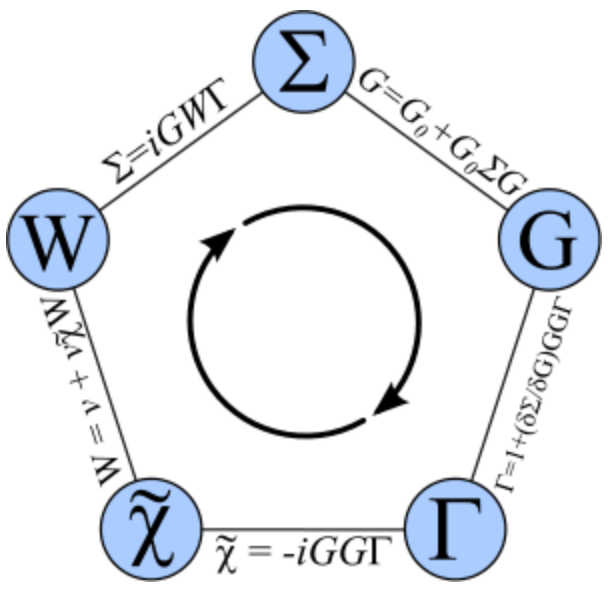
\includegraphics[height=2.5in,width=3.2in,viewport=0 0 680 600,clip]{Figures/GW_Hedin_eq.png}
\caption{\small \textrm{The various physical quantities are interrelated by Hedin equation.}}%
\label{GW_Hedin_eq}
\end{figure} 
}

\section{准粒子与\rm{GW~}近似}
\frame
{
	\frametitle{准粒子图像}
	粒子\textrm{Green's function~}经\textrm{Fourier~}变换,称为谱表示(\textrm{Lehmann~}表示)
	\begin{displaymath}
		G(\vec r,\vec r^{\prime};\omega)=\sum_i\frac{\Psi_i(\vec r,\omega)\Psi_i^{\dag}(\vec r^{\prime},\omega)}{\omega-\varepsilon_i+\mathrm{i}\eta\mathrm{sign}(\varepsilon_i-\mu)}\qquad\eta\rightarrow0^{+}
	\end{displaymath}
	\textcolor{blue}{这里$\Psi_i$满足准粒子方程}
	\begin{displaymath}
		H_0(r)\Psi_i(\vec r,\omega)+\int\mathrm{d}^3r\Sigma(\vec r,\vec r^{\prime};\omega)\Psi_i(\vec r^{\prime},\omega)=\varepsilon_i(\omega)\Psi_i(\vec r,\omega)
	\end{displaymath}
	\textcolor{purple}{准粒子方程的特点}
	\begin{itemize}
		\item 能量本征值\textcolor{red}{$\varepsilon_i$是复数}
		\item 自能\textcolor{red}{$\Sigma$是非\textrm{Hermitian}}
		\item 准粒子波函数\textcolor{red}{$\Psi_i$是非正交的}
	\end{itemize}
}

\frame
{
	\frametitle{准粒子图像}
	如果准粒子能量本征值$\varepsilon_i(\omega_i)$,满足$\omega_i=\Re\varepsilon_i(\omega_i)$
	\vskip 5pt
	当能量虚部$\Im\varepsilon_i(\omega_i)$很小,\textcolor{violet}{对应的\textrm{Green's function~}虚部在此能量出现峰值,该准粒子态的寿命$1/\Im\varepsilon_i(\omega_i)$}
	\vskip 5pt
	对于无相互作用粒子体系,\textcolor{blue}{自能$\Sigma$是\textrm{Hermitian}},\textcolor{red}{能量本征值是实数,处于准粒子定态}
\begin{figure}[h!]
\centering
\vspace*{-0.1in}
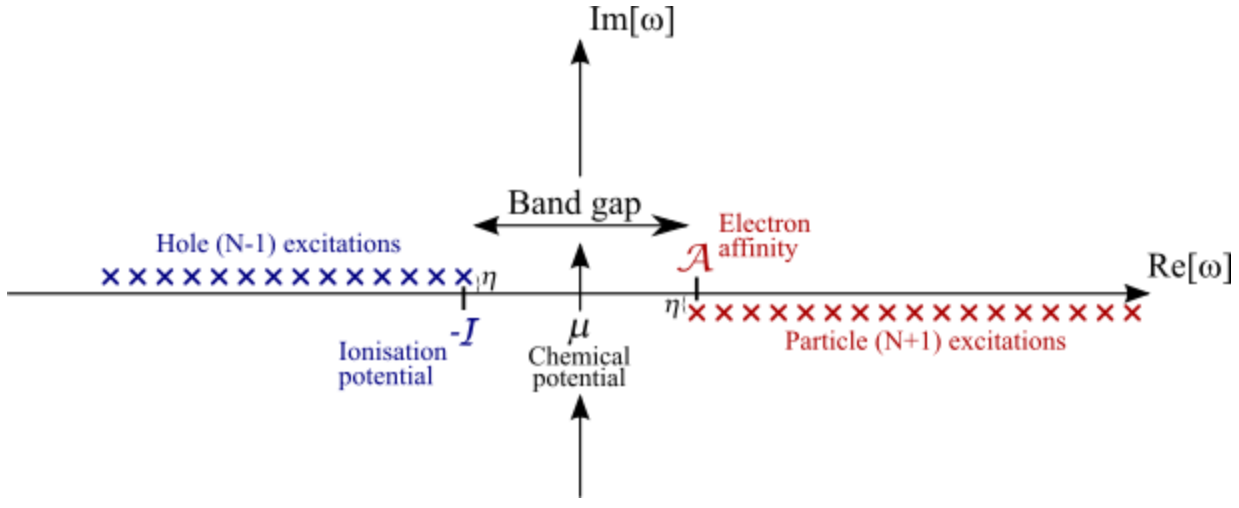
\includegraphics[height=1.3in,width=3.5in,viewport=0 0 1250 520,clip]{Figures/GW_Quasiparticle.png}
\caption{\small \textrm{Schematic representation of the location of the poles of the time-ordered Green's function.}}%
\label{GW_Quasiparticle}
\end{figure} 
}

\frame
{
	\frametitle{粒子数表象下的谱表示}
利用二次量子化,准粒子\textrm{Green's function~}的谱表示可以表示为
\begin{displaymath}
	G(\vec r,\vec r^{\prime};\omega)=\int_{-\infty}^{\mu}\mathrm{d}\omega^{\prime}\frac{A(\vec r,\vec r^{\prime};\omega^{\prime})}{\omega-\omega^{\prime}-\mathrm{i}\delta}+\int_{\mu}^{+\infty}\mathrm{d}\omega^{\prime}\frac{A(\vec r,\vec r^{\prime};\omega^{\prime})}{\omega-\omega^{\prime}+\mathrm{i}\delta}
\end{displaymath}
这里谱函数(\textrm{spectral function})$A$的定义为
\begin{displaymath}
	\begin{aligned}
		A(\vec r,\vec r^{\prime};\omega)=&-\frac1{\pi}\Im G(\vec r,\vec r^{\prime};\omega)\textrm{sign}(\omega-\mu)\\
		=&\sum_ih_i(\vec r)h_i^{\ast}(\vec r^{\prime})\delta[\omega-\mu+e(N-1,i)]\\
		&+\sum_ip_i^{\ast}(\vec r)h_i(\vec r^{\prime})\delta[\omega-\mu-e(N+1,i)]
	\end{aligned}
\end{displaymath}
其中
\begin{displaymath}
	\begin{aligned}
		h_i(\vec r)=\langle N-1,i|\hat{\psi}(\vec r,0)|N\rangle\\
		p_i(\vec r)=\langle N+1,i|\hat{\psi}^{\dag}(\vec r,0)|N\rangle
	\end{aligned}
\end{displaymath}
}

\frame
{
	\frametitle{粒子数表象下的谱表示}
	$|N\pm1,i\rangle$表示$N\pm1$个电子本征态,由此可得激发能(正值)
	\begin{displaymath}
		e(N\pm1,i)=E(N\pm1,i)-E(N\pm1)
	\end{displaymath}
	其中$E(N\pm1)$是$N\pm1$个电子的基态能量
	\vskip 5pt
	$\mu$是化学势,定义为
	\begin{displaymath}
		\begin{aligned}
			\mu=&E(N+1)-E(N)\\
			=&E(N)-E(N-1)
		\end{aligned}
	\end{displaymath}
	\textcolor{red}{\textrm{Green's function~}的极点的物理意义:~}\textcolor{blue}{$N\pm1$电子的激发能}\\即$\Re\varepsilon_i(\omega_i)$对应$N\pm1$电子的激发能\\
	根据\textrm{Dyson~}方程,谱函数与自能的关系
	\begin{displaymath}
		\begin{aligned}
			\begin{aligned}
				A(\omega)=&\frac1{\pi}\sum_i|\Im G_i(\omega)|\\
				=&\frac1{\pi}\sum_i\frac{\Im\Sigma_i(\omega)}{|\omega-\varepsilon_i-\Re\Delta\Sigma_i(\omega)|^2+|\Im\Sigma_i(\omega)|^2}
			\end{aligned}
		\end{aligned}
	\end{displaymath}
}

\frame
{
	\frametitle{准粒子图像}
	谱函数(态密度)$A$的特点
	\begin{itemize}
		\item 峰位对应于准粒子能量$\varepsilon_i^{\mathrm{QP}}$
			\begin{displaymath}
				\begin{aligned}
					\varepsilon_i^{\mathrm{QP}}=&\varepsilon_i+\Re\Delta\Sigma_i(\varepsilon_i^{\mathrm{QP}})\\
					=&\varepsilon_i+\Re\Delta\Sigma_i(\varepsilon_i)+(\varepsilon_i^{\mathrm{QP}}-\varepsilon_i)\frac{\partial\Re\Delta\Sigma_i(\varepsilon_i)}{\partial\omega}\\
					=&\varepsilon_i+Z_i\Re\Delta\Sigma_i(\varepsilon_i)
				\end{aligned}
			\end{displaymath}
		这里$Z_i$称为重整化因子(\textrm{The renormalization factor})
			\begin{displaymath}
				Z_i=\left[ 1-\frac{\partial\Re\Delta\Sigma_i(\varepsilon_i^{\mathrm{QP}})}{\partial\omega} \right]<1
			\end{displaymath}
		\item 准粒子峰的寿命$1/|\Im\Sigma_i(\omega_i)|$
	\end{itemize}
%\begin{figure}[h!]
%\centering
%\vspace*{-0.1in}
%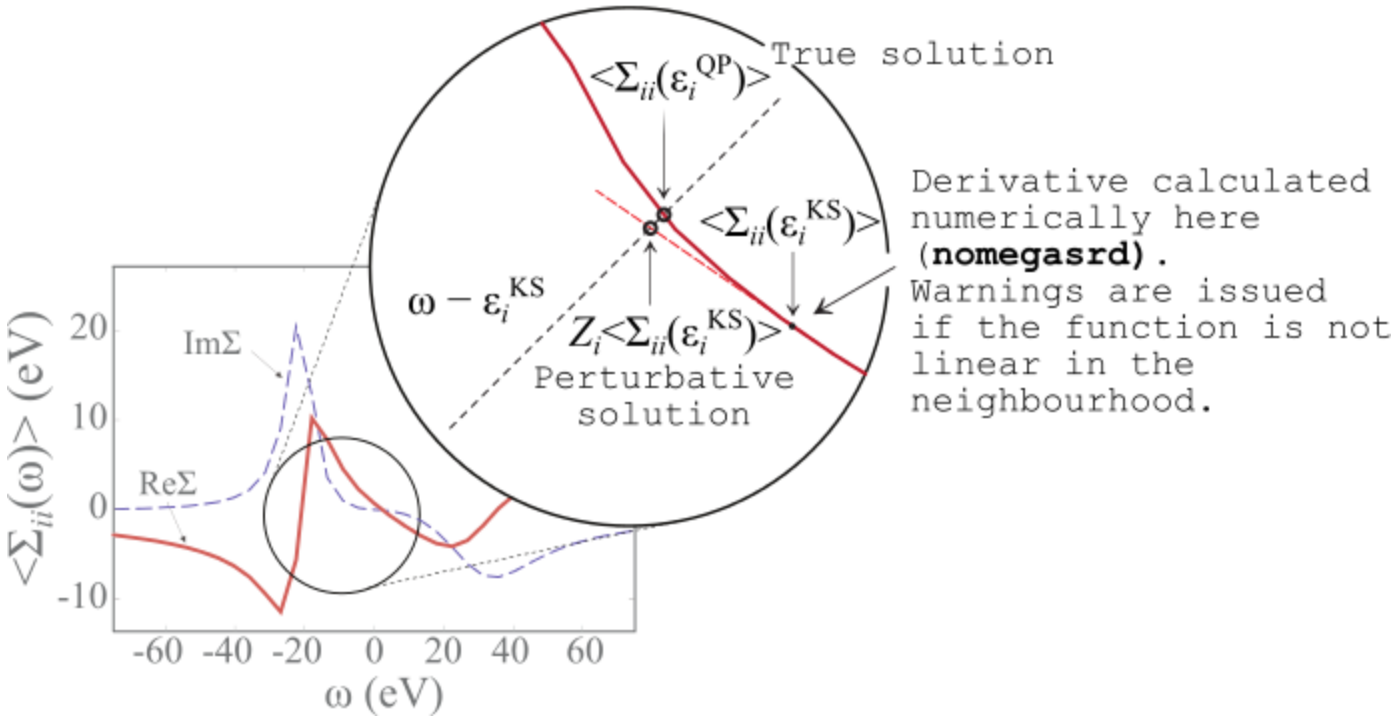
\includegraphics[height=0.55in,width=1.1in,viewport=0 0 1400 720,clip]{Figures/GWA_perturbation.png}
%\caption{\fontsize{7.5pt}{6.2pt}\selectfont{\textrm{Based on DFT, The renormalization factor corresponds to making a Taylor expansion of the self-energy matrix element around the KS energy.}}}%
%\label{GWA_perturbation}
%\end{figure} 
}

\section{\rm{GWA~}近似}
\frame
{
	\frametitle{\textrm{GWA~}近似}
	\begin{itemize}
		\item \textcolor{blue}{\textrm{GWA~}的重要近似}:~\textcolor{red}{忽略顶角函数$\Lambda(\mathbf{1},\mathbf{2},\mathbf{3})=\delta(\mathbf{1}-\mathbf{2})\delta(\mathbf{2}-\mathbf{3})$}
\begin{figure}[h!]
\centering
\vspace*{-0.2in}
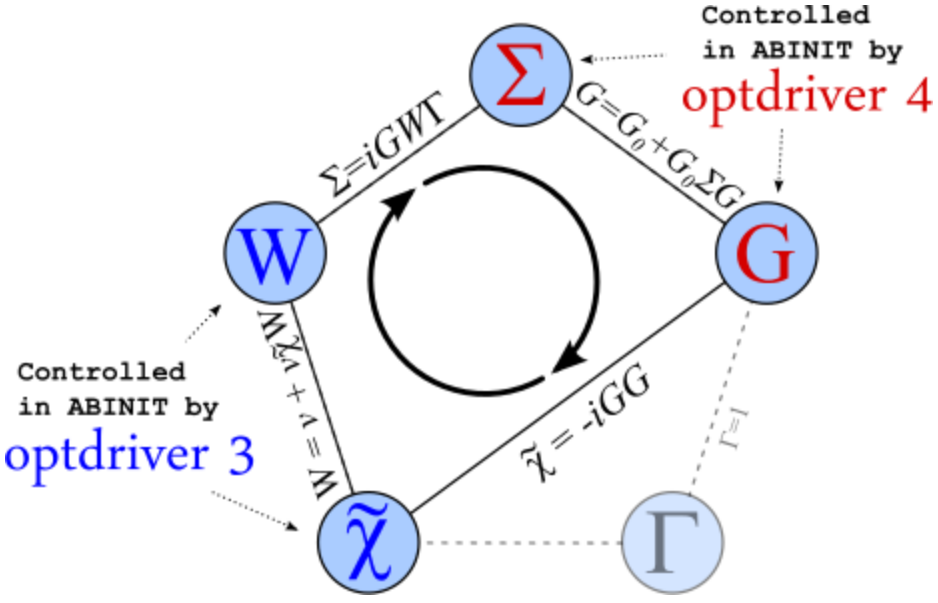
\includegraphics[height=2.5in,width=3.7in,viewport=0 0 950 660,clip]{Figures/GWA_Hedin_eq.png}
\caption{\small \textrm{The approximated vertex leads to a considerable simplification in the Hedin equation.}}%
\label{GWA_Hedin_eq}
\end{figure} 
	\end{itemize}
}

\frame
{
	\frametitle{\textrm{GWA~}的极化函数与\textrm{RPA}}
	为了计算屏蔽\textrm{Coulomb~}相互作用$W$,必须先计算$P$,一般采用无规相近似(\textrm{the Random Phase approximation, RPA}),用无相互作用\textrm{Green's function~}$G_0$,忽略顶角函数
	\begin{displaymath}
		\begin{aligned}
			\chi(\vec r,\vec r^{\prime};\omega)=&\sum_{\mathrm{spin}}\sum_{\vec k,n}^{\mathrm{occ}}\sum_{\vec k^{\prime},n^{\prime}}^{\mathrm{unocc}}\psi_{\vec k,n}^{\ast}(\vec r)\psi_{\vec k^{\prime},n^{\prime}}(\vec r)\psi_{\vec k^{\prime},n^{\prime}}^{\ast}(\vec r^{\prime})\psi_{\vec k,n}(\vec r^{\prime})\\
			&\times\left\{ \frac1{\omega-\varepsilon_{\vec k^{\prime},n^{\prime}}+\varepsilon_{\vec k,n}+\mathrm{i}\delta}+\frac1{\omega+\varepsilon_{\vec k^{\prime},n^{\prime}}-\varepsilon_{\vec k,n}-\mathrm{i}\delta} \right\}
		\end{aligned}
	\end{displaymath}
	作\textrm{Fourier~}变换,可有极化函数矩阵元
	\fontsize{7.5pt}{6.2pt}\selectfont{\begin{displaymath}
		\begin{aligned}
			\chi_{\vec G_1,\vec G_2}^0(\vec q,\omega)=&\sum_{\mathrm{spin}}\sum_{\vec k}\sum_n^{\mathrm{occ}}\sum_m^{\mathrm{unocc}}\langle\vec k,n|\mathrm{e}^{\mathrm{i}(\vec q+\vec G_1)\cdot\vec r}|\vec k+\vec q,m\rangle\langle\vec k+\vec q,m|\mathrm{e}^{-\mathrm{i}(\vec q+\vec G_2)\cdot\vec r}|\vec k,n\rangle\\
			&\times\left\{ \frac1{\omega-\varepsilon_{\vec k+\vec q,m}+\varepsilon_{\vec k,n}+\mathrm{i}\delta}+\frac1{\omega+\varepsilon_{\vec k+\vec q,m}-\varepsilon_{\vec k,n}-\mathrm{i}\delta} \right\}
		\end{aligned}
	\end{displaymath}}
}

\frame
{
	\frametitle{\textrm{GWA~}近似的自能交换与相关}
	\begin{itemize}
		\item \textcolor{blue}{\textrm{GWA~}的本质可以看作是\textrm{Hartree-Fock~}近似推广到引入动态屏蔽\textrm{Coulomb~}相互作用}\\
			\textcolor{red}{在\textrm{GWA~}中,裸的\textrm{Coulomb~}势$v$变成屏蔽相互作用$W$}
			\begin{displaymath}
				\Sigma(\mathbf{1},\mathbf{2})=\mathrm{i}G(\mathbf{1},\mathbf{2})W(\mathbf{1},\mathbf{2})
			\end{displaymath}
	忽略顶角函数的贡献,经\textrm{Fourier~}变换,\textrm{GWA~}的自能计算
			\begin{displaymath}
				\Sigma(\vec r,\vec r^{\prime};\omega)=\frac{\mathrm{i}}{2\pi}\int\mathrm{d}\omega^{\prime}G(\vec r,\vec r^{\prime};\omega+\omega^{\prime})W(\vec r,\vec r^{\prime};\omega^{\prime})
			\end{displaymath}
		\item \textrm{Green's function~}理论中,交换-相关势的表示
			\vskip 3pt
		注意到\textrm{Hartree-Fock~}中交换势的表示为
			\begin{displaymath}
				\Sigma^{\mathrm{x}}(\vec r,\vec r^{\prime})=-\sum_{\vec k,n}^{\mathrm{occ}}\psi_{\vec k,n}(\vec r)\psi_{\vec k,n}^{\ast}(\vec r^{\prime})v(\vec r-\vec r^{\prime})
			\end{displaymath}
	\end{itemize}
}

\frame
{
	\frametitle{\textrm{GWA~}近似的自能交换与相关}
			\textcolor{blue}{对于无相互作用体系的$G_0$},\textcolor{violet}{自能交换部分}\textcolor{blue}{表示为}
			\begin{displaymath}
				\Sigma^{\mathrm{x}}(\vec r,\vec r^{\prime};t-t^{\prime})=\mathrm{i}G(\vec r,\vec r^{\prime};t-t^{\prime})v(\vec r-\vec r^{\prime})\delta(t-t^{\prime})
			\end{displaymath}
			\textcolor{blue}{对于无相互作用体系的$G_0$},\textcolor{violet}{自能相关部分的虚部}\textcolor{blue}{可以表示为}
	\fontsize{9pt}{6.2pt}\selectfont{\begin{displaymath}
				\hspace*{-8pt}
				\begin{aligned}
					&\Im\Sigma^{\mathrm{c}}(\vec r,\vec r^{\prime};\omega\leqslant\mu)=\pi\sum_{\vec k,n}^{\mathrm{occ}}\psi_{\vec k,n}(\vec r)\psi_{\vec k,n}^{\ast}(\vec r^{\prime})\Im W^{\mathrm{c}}(\vec r,\vec r^{\prime};\varepsilon_{\vec k,n}-\omega)\theta(\varepsilon_{\vec k,n}-\omega)\\
					&\Im\Sigma^{\mathrm{c}}(\vec r,\vec r^{\prime};\omega>\mu)=-\pi\sum_{\vec k,n}^{\mathrm{unocc}}\psi_{\vec k,n}(\vec r)\psi_{\vec k,n}^{\ast}(\vec r^{\prime})\Im W^{\mathrm{c}}(\vec r,\vec r^{\prime};\omega-\varepsilon_{\vec k,n})\theta(\omega-\varepsilon_{\vec k,n})
				\end{aligned}
			\end{displaymath}}
			这里$W^{\mathrm{c}}=W-v$,其频率表示
			\begin{displaymath}
				W^{\mathrm{c}}(\vec r,\vec r^{\prime};\omega)=\int_{-\infty}^0\mathrm{d}\omega^{\prime}\frac{D(\vec r,\vec r^{\prime};\omega^{\prime})}{\omega-\omega^{\prime}-\mathrm{i}\delta}+\int_0^{\infty}\mathrm{d}\omega^{\prime}\frac{D(\vec r,\vec r^{\prime};\omega^{\prime})}{\omega-\omega^{\prime}+\mathrm{i}\delta}
			\end{displaymath}
}

\frame
{
	\frametitle{\textrm{GWA~}近似的自能交换与相关}
	\textcolor{blue}{$D$称为等离子频率,是关于$\omega$是反对称的},正比于$W$的虚部
	\begin{displaymath}
		\begin{aligned}
			&D(\vec r,\vec r^{\prime};\omega)=-\frac1{\pi}\Im W^{\mathrm{c}}(\vec r,\vec r^{\prime};\omega)\textrm{sign}(\omega)\\
			&D(\vec r,\vec r^{\prime};\omega)=-D(\vec r,\vec r^{\prime};\omega)
		\end{aligned}
	\end{displaymath}
	\textrm{GWA~}的自能相关部分
	\begin{displaymath}
		\Sigma^{\mathrm{c}}(\vec r,\vec r^{\prime};\omega)=\int_{-\infty}^{\mu}\mathrm{d}\omega^{\prime}\frac{\Gamma(\vec r,\vec r^{\prime};\omega^{\prime})}{\omega-\omega^{\prime}-\mathrm{i}\delta}+\int_{\mu}^{\infty}\mathrm{d}\omega^{\prime}\frac{\Gamma(\vec r,\vec r^{\prime};\omega^{\prime})}{\omega-\omega^{\prime}+\mathrm{i}\delta}
	\end{displaymath}
	其中
	\begin{displaymath}
		\Gamma(\vec r,\vec r^{\prime};\omega)=-\frac1{\pi}\Im\Sigma^{\mathrm{c}}(\vec r,\vec r^{\prime};\omega)\textrm{sign}(\omega-\mu)
	\end{displaymath}
	\textcolor{blue}{自能相关部分$\Sigma^{\mathrm{c}}$的实部由积分主值得到}
}

\frame
{
	\frametitle{\textrm{GWA~}近似的自能交换与相关}
	综上所述,自能可分解成\textcolor{purple}{屏蔽交换项$\Sigma_{\mathrm{SEX}}$}和\textcolor{purple}{相关孔项$\Sigma_{\mathrm{COH}}$}\\(\textrm{COHSEX})其实部可表示为
	\begin{displaymath}
		\begin{aligned}
			&\Re\Sigma_{\mathrm{SEX}}(\vec r,\vec r^{\prime};\omega)=-\sum_i^{\mathrm{occ}}\psi_i(\vec r)\psi_i^{\ast}(\vec r^{\prime})\Re W(\vec r,\vec r^{\prime};\omega-\varepsilon_i)\\
			&\Re\Sigma_{\mathrm{COH}}(\vec r,\vec r^{\prime};\omega)=\sum_i\psi_i(\vec r)\psi_i^{\ast}(\vec r^{\prime})\mathscr{P}\int_0^{+\infty}\mathrm{d}\omega^{\prime}\frac{D(\vec r,\vec r^{\prime};\omega^{\prime})}{\omega-\varepsilon_i-\omega^{\prime}}\\
		\end{aligned}
	\end{displaymath}
	当关注的能量$\omega$接近\textrm{Fermi~}能级,矩阵元$\langle\psi|\Re\Sigma_{\mathrm{COH}}(\omega)|\psi\rangle$\textcolor{blue}{计算了接近$\omega$的能量本征态的贡献},令$\omega-\varepsilon_i=0$,
	\begin{displaymath}
		\Re\Sigma_{\mathrm{COH}}(\vec r,\vec r^{\prime})=\frac12\delta(\vec r-\vec r^{\prime})W^{\mathrm{c}}(\vec r,\vec r^{\prime};0)
	\end{displaymath}
	\textcolor{red}{这是简化的准粒子相互作用能,因子$1/2$来自绝热开启相互作用,静态\textrm{COHSEX~}近似下,$\Sigma_{\mathrm{COH}}$是局域的}
}

%\frame
%{
%\frametitle{发展统一理论框架下的材料计算程序}
%\begin{itemize}
%	\item
%\end{itemize}
%}

%\appendix
%------------------------------------------------------------------------Reference----------------------------------------------------------------------------------------------
%\begin{thebibliography}{99}
%-----------------------------------------------------------------------------------------------------------------------------------------------------------------------%
%\frame
%{
%\frametitle{主要参考文献}
%{\small
%\bibitem{Singh_Book}\textrm{D. J. Singh. \textit{Plane Wave, PseudoPotential and the LAPW method} (Kluwer Academic, Boston,USA, 1994)}					%
%  \nocite{*}																				%
%}
%}
%\end{thebibliography}
\begin{thebibliography}{99}
\frame
{
\frametitle{主要参考文献}
{\small
%	\bibitem{Huang_Han}黄昆\:原著、韩汝琦\:改编, {\textit{固体物理学}}\:高等教育出版社, 北京, 1988
%	\bibitem{Xie_Lu}谢希德、陆栋\:主编, {\textit{固体能带理论}}\:复旦大学出版社, 上海, 1998
        \bibitem{Inkson_Book}\textrm{J. C. Inkson. \textit{Many-Body Theory of Solids: An Introduction} (Plenum Press, New York, USA, 1984)}
	\bibitem{Comp_Method}\textrm{V. V. Nemoshkalenko and V. N. Antonov. \textit{Computational Methods in Solid State Physics} (Gordon and Breach Science Publisher, Amsterdam, The Netherlands, 1998)}
	\bibitem{RPP61-237_1998}\fontsize{9.2pt}{3.9pt}\selectfont{\textcolor{red}{\frame{\textrm{F. Aryasetiawan and O. Gunnarsson \textit{Rep. Prog. Phys.}, \textbf{61} (1998), 237}}}}
	\bibitem{PR-139-A796_1965}\textrm{L. Hedin. \textit{Phys. Rev.}, \textbf{139} (1965), A796}
%	\bibitem{SSC114-15_2000}\textrm{E. Sj\"ostedt, L. Nordstr\"om and D. J. Singh. \textit{Solid State Commun.}, \textbf{114} (2000), 15}
	\bibitem{Bruus_Flensberg}\textrm{H. Bruus and K. Flensberg. \textit{Many-Body Quantum Theory in Condensed Matter Physics: An Introduction} (Oxford University Press, U.K., 2004)}
}
\nocite*{}
}
\end{thebibliography}
%{\small
%\phantomsection\addcontentsline{toc}{section}{Bibliography}	 %直接调用\addcontentsline命令可能导致超链指向不准确,一般需要在之前调用一次\phantomsection命令加以修正	%
%\bibliography{Myref}																			%
%\bibliographystyle{mybib}																		%
%  \nocite{*}																				%
%}
%-----------------------------------------------------------------------------------------------------------------------------------------------------------------------%


%-----------------------------------------------------------Beamer下不建议使用bib,因为涉及分页--------------------------------------------------------------------------%
%{\small
%\phantomsection\addcontentsline{toc}{section}{Bibliography}	 %直接调用\addcontentsline命令可能导致超链指向不准确,一般需要在之前调用一次\phantomsection命令加以修正	%
%\bibliography{Myref}																			%
%\bibliographystyle{mybib}																		%
%  \nocite{*}																				%
%}

%------------------------------------------------------------------------------------------------------------------------------------------------------------------------------%

%-------------------------------------------------------------------------Thanks------------------------------------------------------------------------------------------------
%\section{致谢}
%\frame
%{
%\frametitle{致$\quad$谢}
%\begin{itemize}
%    \setlength{\itemsep}{20pt}
%  \item 感谢本团队高兴誉、吴泉生、宋红州等各位老师参与的讨论
%  \item 感谢莫所长、宋主任以及软件中心各位老师和同事
%  \item 感谢王崇愚先生的帮助
%\end{itemize}
%}

\logo{}									%不显示logo
\frame
{
\vskip 60 pt
%\hskip 10pt \textcolor{blue}{\Huge 感谢答辩委员会各位老师\,\textrm{!}}\\
\vskip 35 pt
\hskip 60pt \textcolor{blue}{\Huge 谢谢大家\:!}
%\vskip 15 pt
%\hskip 40pt \textcolor{blue}{\Huge \textrm{for your attention\:!}}
}

%-------------------------------------------------------------------------------------------------------------------------------------------------------------------------------

\clearpage
%\end{CJK*}
\end{document}
